\newpage
\section{Additional information}
\subsection*{Script \& Code}
Script and code created and used can be found at:\\
http:$\backslash$$\backslash$github.com$\backslash$DannyArends\\
http:$\backslash$$\backslash$github.com$\backslash$DannyArends$\backslash$rqtl-mqm\\
http:$\backslash$$\backslash$github.com$\backslash$DannyArends$\backslash$MolgenisInterface\\

\subsection*{Additional tables}
Tables \ref{tbl:tabel1} \& \ref{tbl:tabelCluster} list the dependencies needed to use the software discribed in this thesis. 
The scriptfile QTLanalysis.R ,dependency for functioning of the clusterservice,
can be found inside the molgenispackage.
Tables \ref{tbl:tabel3} \& \ref{tbl:tabel2} made using R/qtl "Map10" dataset, for scanone bootstrapping parameters were: 
500 bootstraps in batches of 50 at a time on a simulated F2 population with \# individuals as stated in column 1 (Table \ref{tbl:tabel2}).
For mqm we used 50 bootstraps in batches of 5 (Table \ref{tbl:tabel3}). Runs were performed using standard setting for each algorithm. 
Profiling code is available at request.\\

\begin{table}[ht]
	\caption{Requirements for using the R/qtl package}
	\centering
	\begin{tabular}{| l | c | }
	\hline
	Operating system(s):&platform independent\\
	Programming languages:&R, C++\\
	Programs:&R 2.8.0\\
	Dependencies:&SNOW\cite{tierney04}\\
	Published using:&GNU 2 licence\\
	\hline
	\end{tabular}
	\label{tbl:tabel1}
\end{table}

\begin{table}[ht]
	\caption{Requirements for using R/qtl on a cluster}
	\centering
	\begin{tabular}{| l | c | }
	\hline
	Operating system(Cluster):&Unix / Linux\\
	Operating system(Webservice):&platform independent\\
	Programs(Cluster):&R 2.8.0\\
	&PBS\\
	Programs(Webservice):&Molgenis 3.3 Distro\\
	&XGAP 1.1\\
	Dependencies(Cluster):&molgenispackage\\
	&R/qtl\\
	&RCurl\cite{Rcurl08}\\
	&QTLanalysis.R\\
	Dependencies(Webservice):&webserver(APACHE)\\
	&database(mySQL)\\
	&Eclipse Ganymede (Developers)\\
	Published using:&GNU 2 licence\\
	\hline
	\end{tabular}
	\label{tbl:tabelCluster}
\end{table}

\begin{table}[ht]
	\caption{Profiling bootstrap analysis of scanone using a QuadCore machine}
	\centering
	\begin{tabular}{| l | l | l | l | l | c | c | c |}
	\hline
	\# Individuals & Single & Ncore=2 & Ncore=3 & Ncore=4 & \%2vs1 & \%3vs1 & \%4vs1\\
	\hline
	\hline
	10 & 83.00 & 68.00 & 65.00 & 65.00 & -18.1\% & -21.7\% & -21.7\%\\
	20 & 91.00 & 72.00 & 67.00 & 67.00 & -20.9\% & -26.4\% & -26.4\%\\
	50 & 118.00 & 84.00 & 76.00 & 74.00 & -28.8\% & -35.6\% & -37.3\%\\
	100	& 161.00 & 104.00 & 90.00 & 85.00 & -35.4\% & -44.1\% & -47.2\%\\
	200	& 251.00 & 146.00 & 118.00 & 107.00 & -41.8\% & -53.0\% & -57.4\%\\
	350	& 377.00 & 204.00 & 158.00 & 138.00 & -45.9\% & -58.1\% & -63.4\%\\
	500	& 501.00 & 261.00 & 198.00 & 169.00 & -47.9\% & -60.5\% & -66.3\%\\
	750	& 709.00 & 359.00 & 263.00 & 220.00 & -49.4\% & -62.9\% & -69.0\%\\
	1000 & 919.00 & 453.00 & 329.00 & 271.00 & -50.7\% & -64.2\% & -70.5\%\\
	2000 & 1754.00 & 840.00 & 593.00 & 477.00 & -52.1\% & -66.2\% & -72.8\%\\
	\hline
	\end{tabular}
	\label{tbl:tabel3}
\end{table}

\begin{table}[ht]
	\caption{Profiling analysis using a DualCore machine}
	\centering
	\begin{tabular}{| l | l | l | l | c |}
	\hline
	\# Individuals &	Method &	Single (sec) &	N.core=2 (sec) & \% Improvement (\%) \\
	\hline
	\hline
	10	& scanone &	103.00 &	85.00 &	17.5\%\\
	20	& scanone &	115.00&	90.00&	21.7\%\\
	50	& scanone &	149.00&	107.00&	28.2\%\\
	100	& scanone &	205.00&	133.00&	35.1\%\\
	200	& scanone &	318.00&	187.00&	41.2\%\\
	350	& scanone &	479.00&	266.00&	44.5\%\\
	500	& scanone &	645.00&	339.00&	47.4\%\\
	750	& scanone &	915.00&	465.00&	49.2\%\\
	1000 & scanone &	1186.00&	555.00&	53.2\%\\
	\hline
	10	&mqm&	143.00&	88.00&	38.5\%\\
	20	&mqm&	177.00&	99.00&	44.1\%\\
	50	&mqm&	211.00&	107.00&	49.3\%\\
	100	&mqm&	237.00&	133.00&	43.9\%\\
	200	&mqm&	347.00&	186.00&	46.4\%\\
	350 &mqm&	501.00&	270.00&	46.1\%\\
	500	&mqm&	646.00&	358.00&	44.6\%\\
	750	&mqm&	962.00&	505.00&	47.5\%\\
	1000 &mqm&	1311.00&	700.00&	46.6\%\\
	\hline
	\end{tabular}
	\label{tbl:tabel2}
\end{table}

\begin{table}[h!t]
	\caption{Profiling scalability of MQM}
	\centering
	\begin{tabular}{| l | l | l | l | l | l | l | l | l |}
	\hline
	\# Ind & \# Chr  & Length Chr & Markers & Stepsize & Stepped chr & Cof Each & Traits & Time (min)\\
	\hline
	\hline
	50 & 10 & 200 & 10*10 & 5 & 0-200 & 0 & 1 & 1.83\\
	100 & 10 & 200 & 10*10 & 5 & 0-200 & 0 & 1 & 2.17\\
	200 & 10 & 200 & 10*10 & 5 & 0-200 & 0 & 1 & 2.91\\
	400 & 10 & 200 & 10*10 & 5 & 0-200 & 0 & 1 & 4.14\\
	800 & 10 & 200 & 10*10 & 5 & 0-200 & 0 & 1 & 7.08\\	
	\hline
	100 & 1 & 200 & 100*1 & 5 & 0-200 & 0 & 1 & 0.48\\
	100 & 5 & 200 & 20*5 & 5 & 0-200 & 0 & 1 & 1.22\\
	100 & 10 & 200 & 10*10 & 5 & 0-200 & 0 & 1 & 2.91\\
	100 & 20 & 200 & 5*20 & 5 & 0-200 & 0 & 1 & 4.17\\
	\hline
	100 & 10 & 50 & 10*10 & 5 & 0-200 & 0 & 1 & 2.28\\
	100 & 10 & 100 & 10*10 & 5 & 0-200 & 0 & 1 & 2.19\\
	100 & 10 & 200 & 10*10 & 5 & 0-200 & 0 & 1 & 2.19\\
	\hline
	100 & 10 & 200 & 10*10 & 1 & 0-200 & 0 & 1 & 9.13\\
	100 & 10 & 200 & 10*10 & 2 & 0-200 & 0 & 1 & 4.81\\
	100 & 10 & 200 & 10*10 & 5 & 0-200 & 0 & 1 & 2.19\\
	100 & 10 & 200 & 10*10 & 10 & 0-200 & 0 & 1 & 1.28\\
	100 & 10 & 200 & 10*10 & 20 & 0-200 & 0 & 1 & 0.82\\
	\hline
	100 & 10 & 200 & 10*10 & 5 & 0-200 & 8 & 1 & 1.7\\
	100 & 10 & 200 & 10*10 & 5 & 0-200 & 5 & 1 & 2.13\\
	100 & 10 & 200 & 10*10 & 5 & 0-200 & 3 & 1 & 3.14\\
	100 & 10 & 200 & 10*10 & 5 & 0-200 & 2 & 1 & 5.94\\
	\hline
	800 & 10 & 200 & 50*10 & 5 & 0-200 & 8 & 1 & 79.29\\
	400 & 10 & 200 & 50*10 & 5 & 0-200 & 8 & 1 & 42.51\\
	100 & 10 & 200 & 50*10 & 5 & 0-200 & 8 & 1 & 14.22\\
	\hline
	\end{tabular}
	\label{tbl:tabel4}
\end{table}

\begin{table}[h!t]
	\caption{R/qtl parameters}
	\centering
	\begin{tabular}{| l | l | }
	\hline
	&\bf QTL mapping method\\
	\hline
	Scanall	&Main scanning interface of R/qtl created by K. Broman et al\\
			&implementing per marker QTL analysis using different models \\
			&and mapping methods.\\
	\hline
	MQMall	&Multiple QTL Mapping algorithm created by R.C. Janssen\\
			&implementing multiple QTL modeling and mapping using normal\\ 
			&distributions.\\
	\hline
	CIMall	&Composite interval mapping created by G. Churchill and \\
			&Senuk Sen\\
	\hline
	&\bf QTL trait model\\
	\hline
	Normal & Used for traits that follow a normal distribution\\
	\hline
	2part & 2-part model\\
	\hline
	Binary & Used for binary traits\\
	\hline
	Non-Parametric & Used when none of the other models fit the trait\\
		&data (least power)\\
	\hline
	&\bf Method of mapping QTLs\\
	\hline
	em & EM Algorithm\\
	\hline
	imp & Imputation\\
	\hline
	hk & Hailey-Knott regression\\
	\hline
	ehk & extended Hailey-Knott\\
	\hline
	mr & Basic marker regression (removing unknowns)\\
	\hline
    mr-imp & marker regression by single imputation of unknown values\\
	\hline
	mr-argmax & Marker regression using the viterbi algorithm to estimate \\
	& unknown values\\
	\hline
	\end{tabular}
	\label{tbl:tabelPARAMS}
\end{table}

\begin{table}[h!t]
	\caption{Taskreporter plugin status codes}
	\centering
	\begin{tabular}{| l | c | c | }
	\hline
	-1	&Red	&An error has occurred.\\
	\hline
	0	&Orange	&Submitted to cluster as a potential job.\\
	\hline
	1	&Yellow	&Job is accepted and queued.\\
	\hline
	2	&Blue	&Job is running.\\
	\hline
	3	&Green	&Job is completed.\\
	\hline
	\end{tabular}
	\label{tbl:tabelSTATUS}
\end{table}
\clearpage
\subsection*{Additional figures}
	\begin{figure}[ht]
	  \hfill
	  \fbox{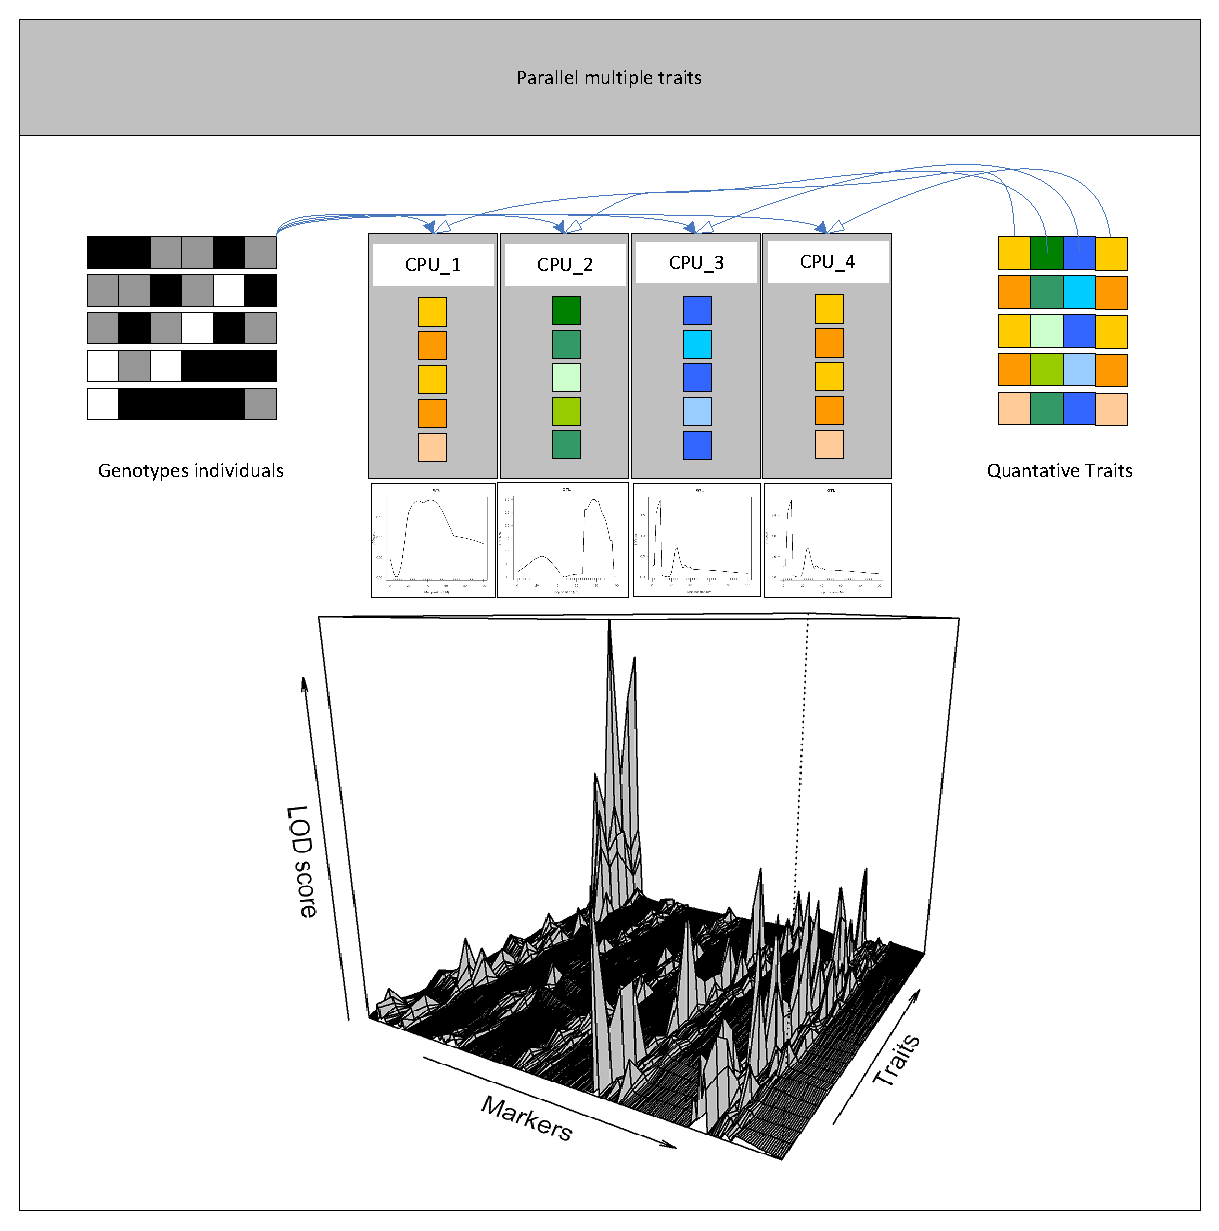
\includegraphics[height=5.0cm,width=10.0cm]{Images/MT_small_newer.eps}}
	  \caption{Overview of the way many endophenotypes are analysed using multiple cores. Tasks are split linearly and distributed across available cores ($Here: \# core = \# traits$, with $traits > cores$ traits are batched into jobs, which are then distributed across cores.)}
	  \label{fig:MTstrait}
	\end{figure}
	
	\begin{figure}[ht]
	  \hfill
	  \fbox{\includegraphics[height=8.0cm,width=12.0cm]{Images/MTperm.eps}}
	  \caption{Overview of the way many endophenotypes permutation using multiple cores. Tasks consist of a single permutation of the data keeping trait correlation intact. Tasks are split linearly and distributed across available cores ($Here: \# core = \# traits$, with $traits > cores$ traits are batched into jobs, which are then distributed across cores.)}
	  \label{fig:MTperm}
	\end{figure}
	
	\begin{figure}[ht]
	  \hfill
	  \fbox{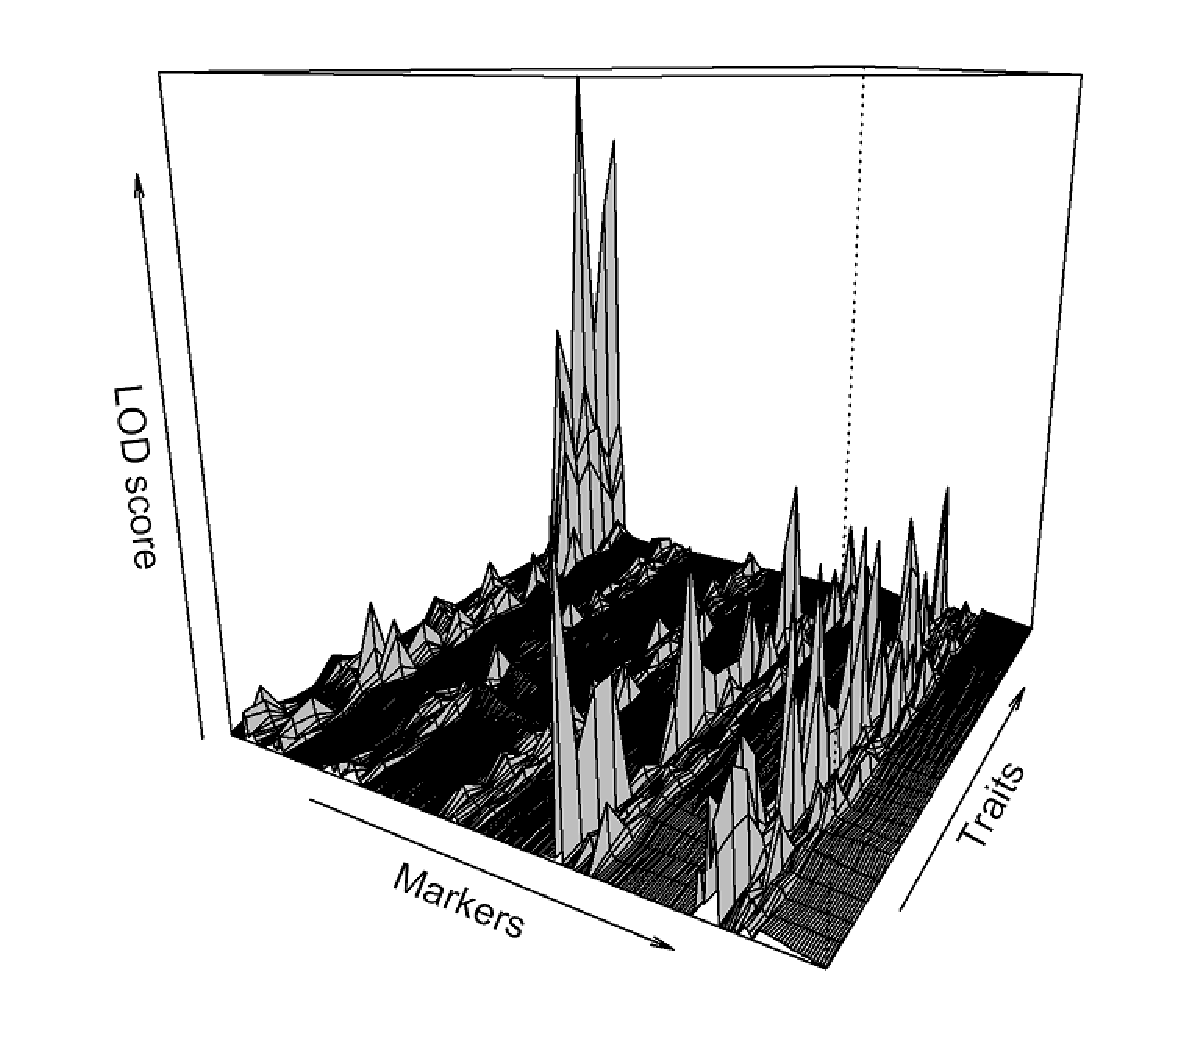
\includegraphics[height=8.0cm,width=12.0cm]{Images/multi3d.eps}}
	  \caption{Example of new ploting routine: Many endophenotypes analyses on 24 traits of the example dataset: "multitrait", displayed in 3D mode}
	  \label{fig:FigureThreeD}
	\end{figure}
	
	\begin{figure}[ht]  
	  \hfill
	  \fbox{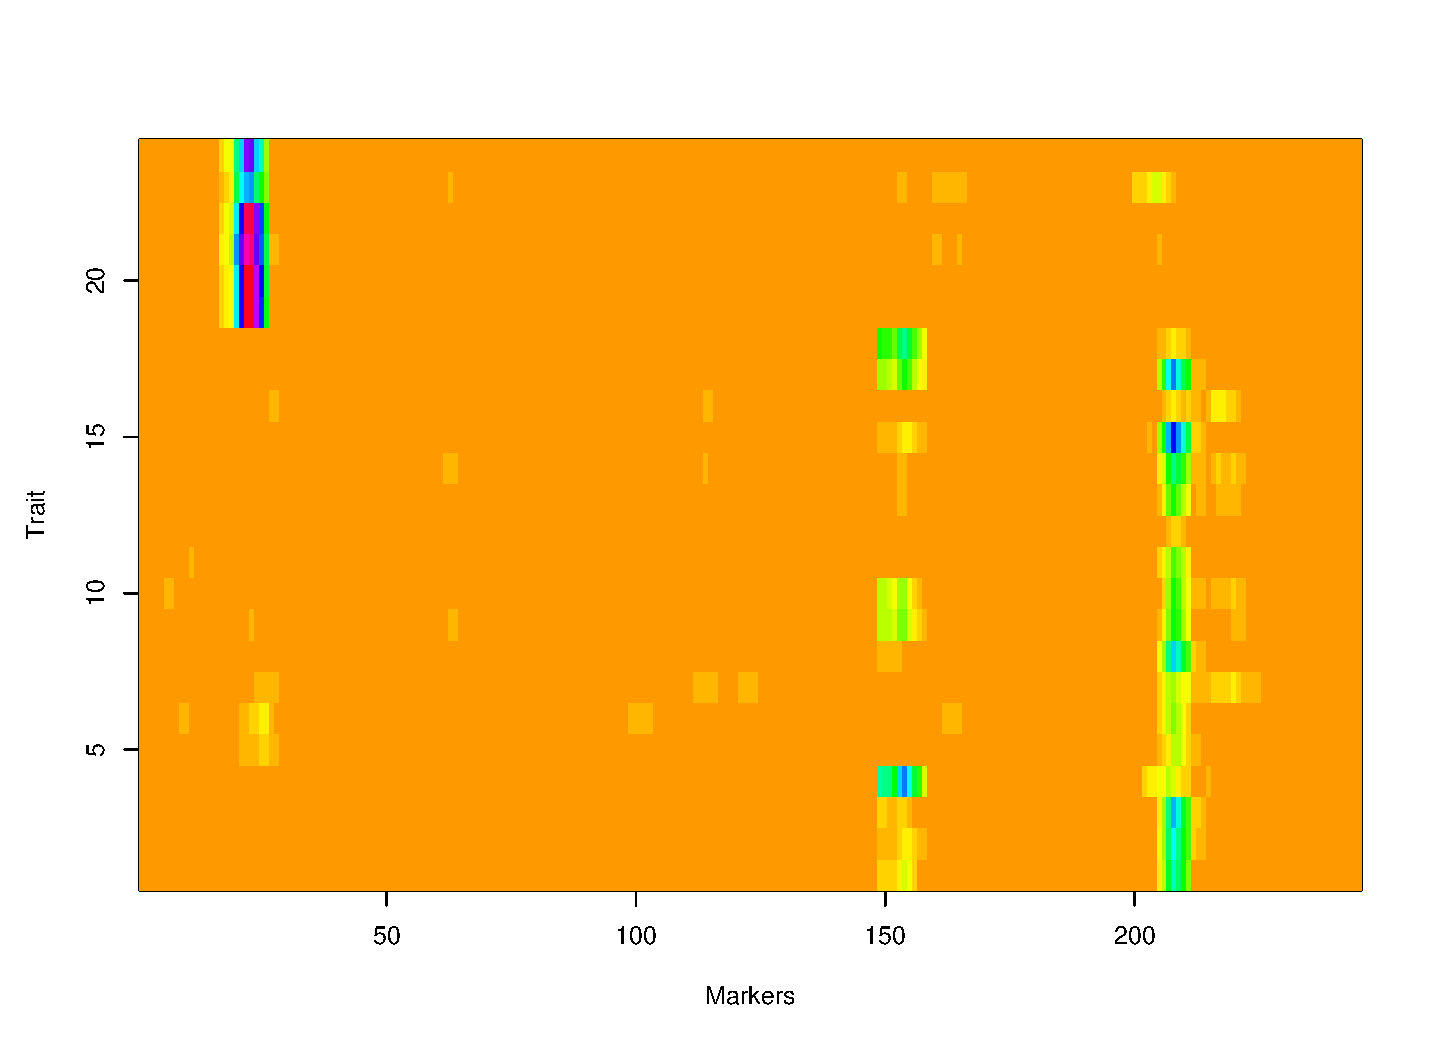
\includegraphics[height=8.0cm,width=12.0cm]{Images/multiHeat.eps}}
	  \caption{Example of new ploting routine: Many endophenotypes analyses analysis on the 24 traits of the example dataset: "multitrait", as a heatmap}
	  \label{fig:FigureHeat}    
	\end{figure}
	
	\begin{figure}[ht]  
	  \hfill
	  \fbox{\includegraphics[height=8.0cm,width=12.0cm]{Images/bootstrap12500.eps}}
	  \caption{Example of new ploting routine: Bootstrap analysis on trait 6 of the example dataset: "multitrait". In this picture the dashed green line represents a 5\% significance threshold, the blue a 10\%.}
	  \label{fig:FigureBoot}
	\end{figure}
	
	\begin{figure}[ht]
	  \hfill
	  \fbox{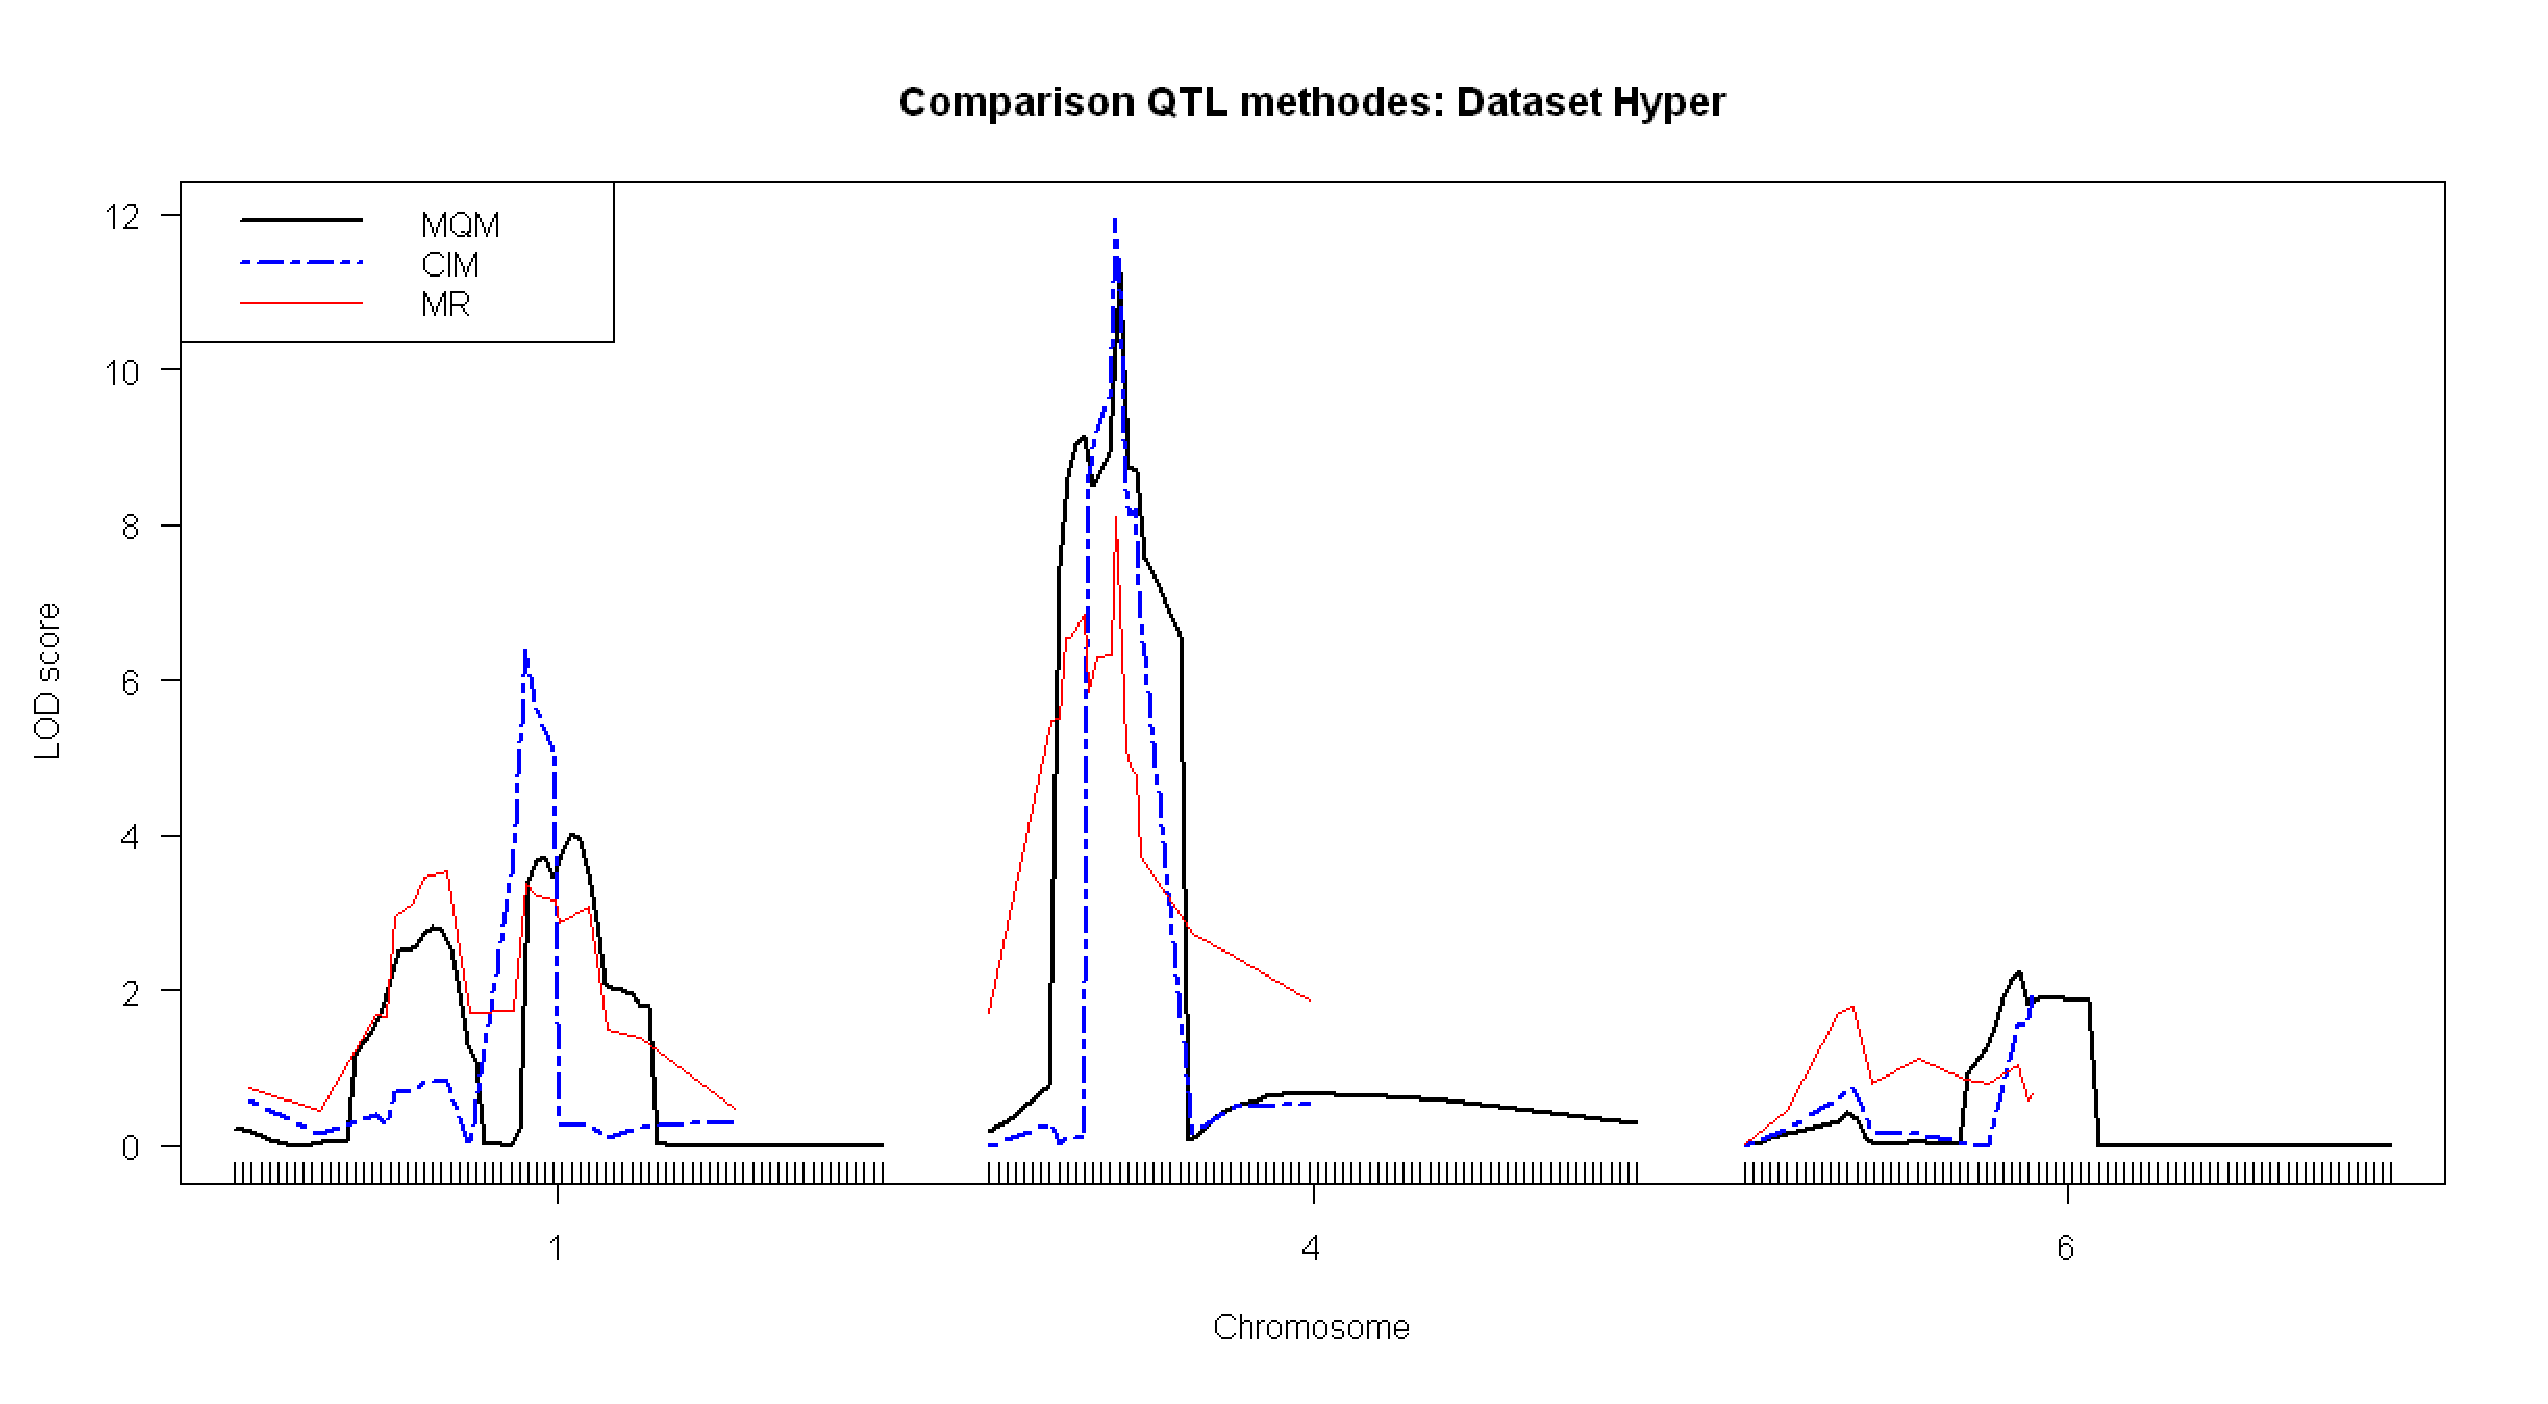
\includegraphics[height=8.0cm,width=12.0cm]{Images/DatasetHyper.eps}}
	  \caption{MQM in comparison with other QTLmapping methods (CIM, MR) using the dataset: "hyper". Using MQM we set cofactors every third marker, and do backward selection using a windowsize of 15 Cm. CIM also uses a window of 15Cm}
	  \label{fig:FigureHyper}
	\end{figure}
	
	\begin{figure}[ht]
	  \hfill
	  \fbox{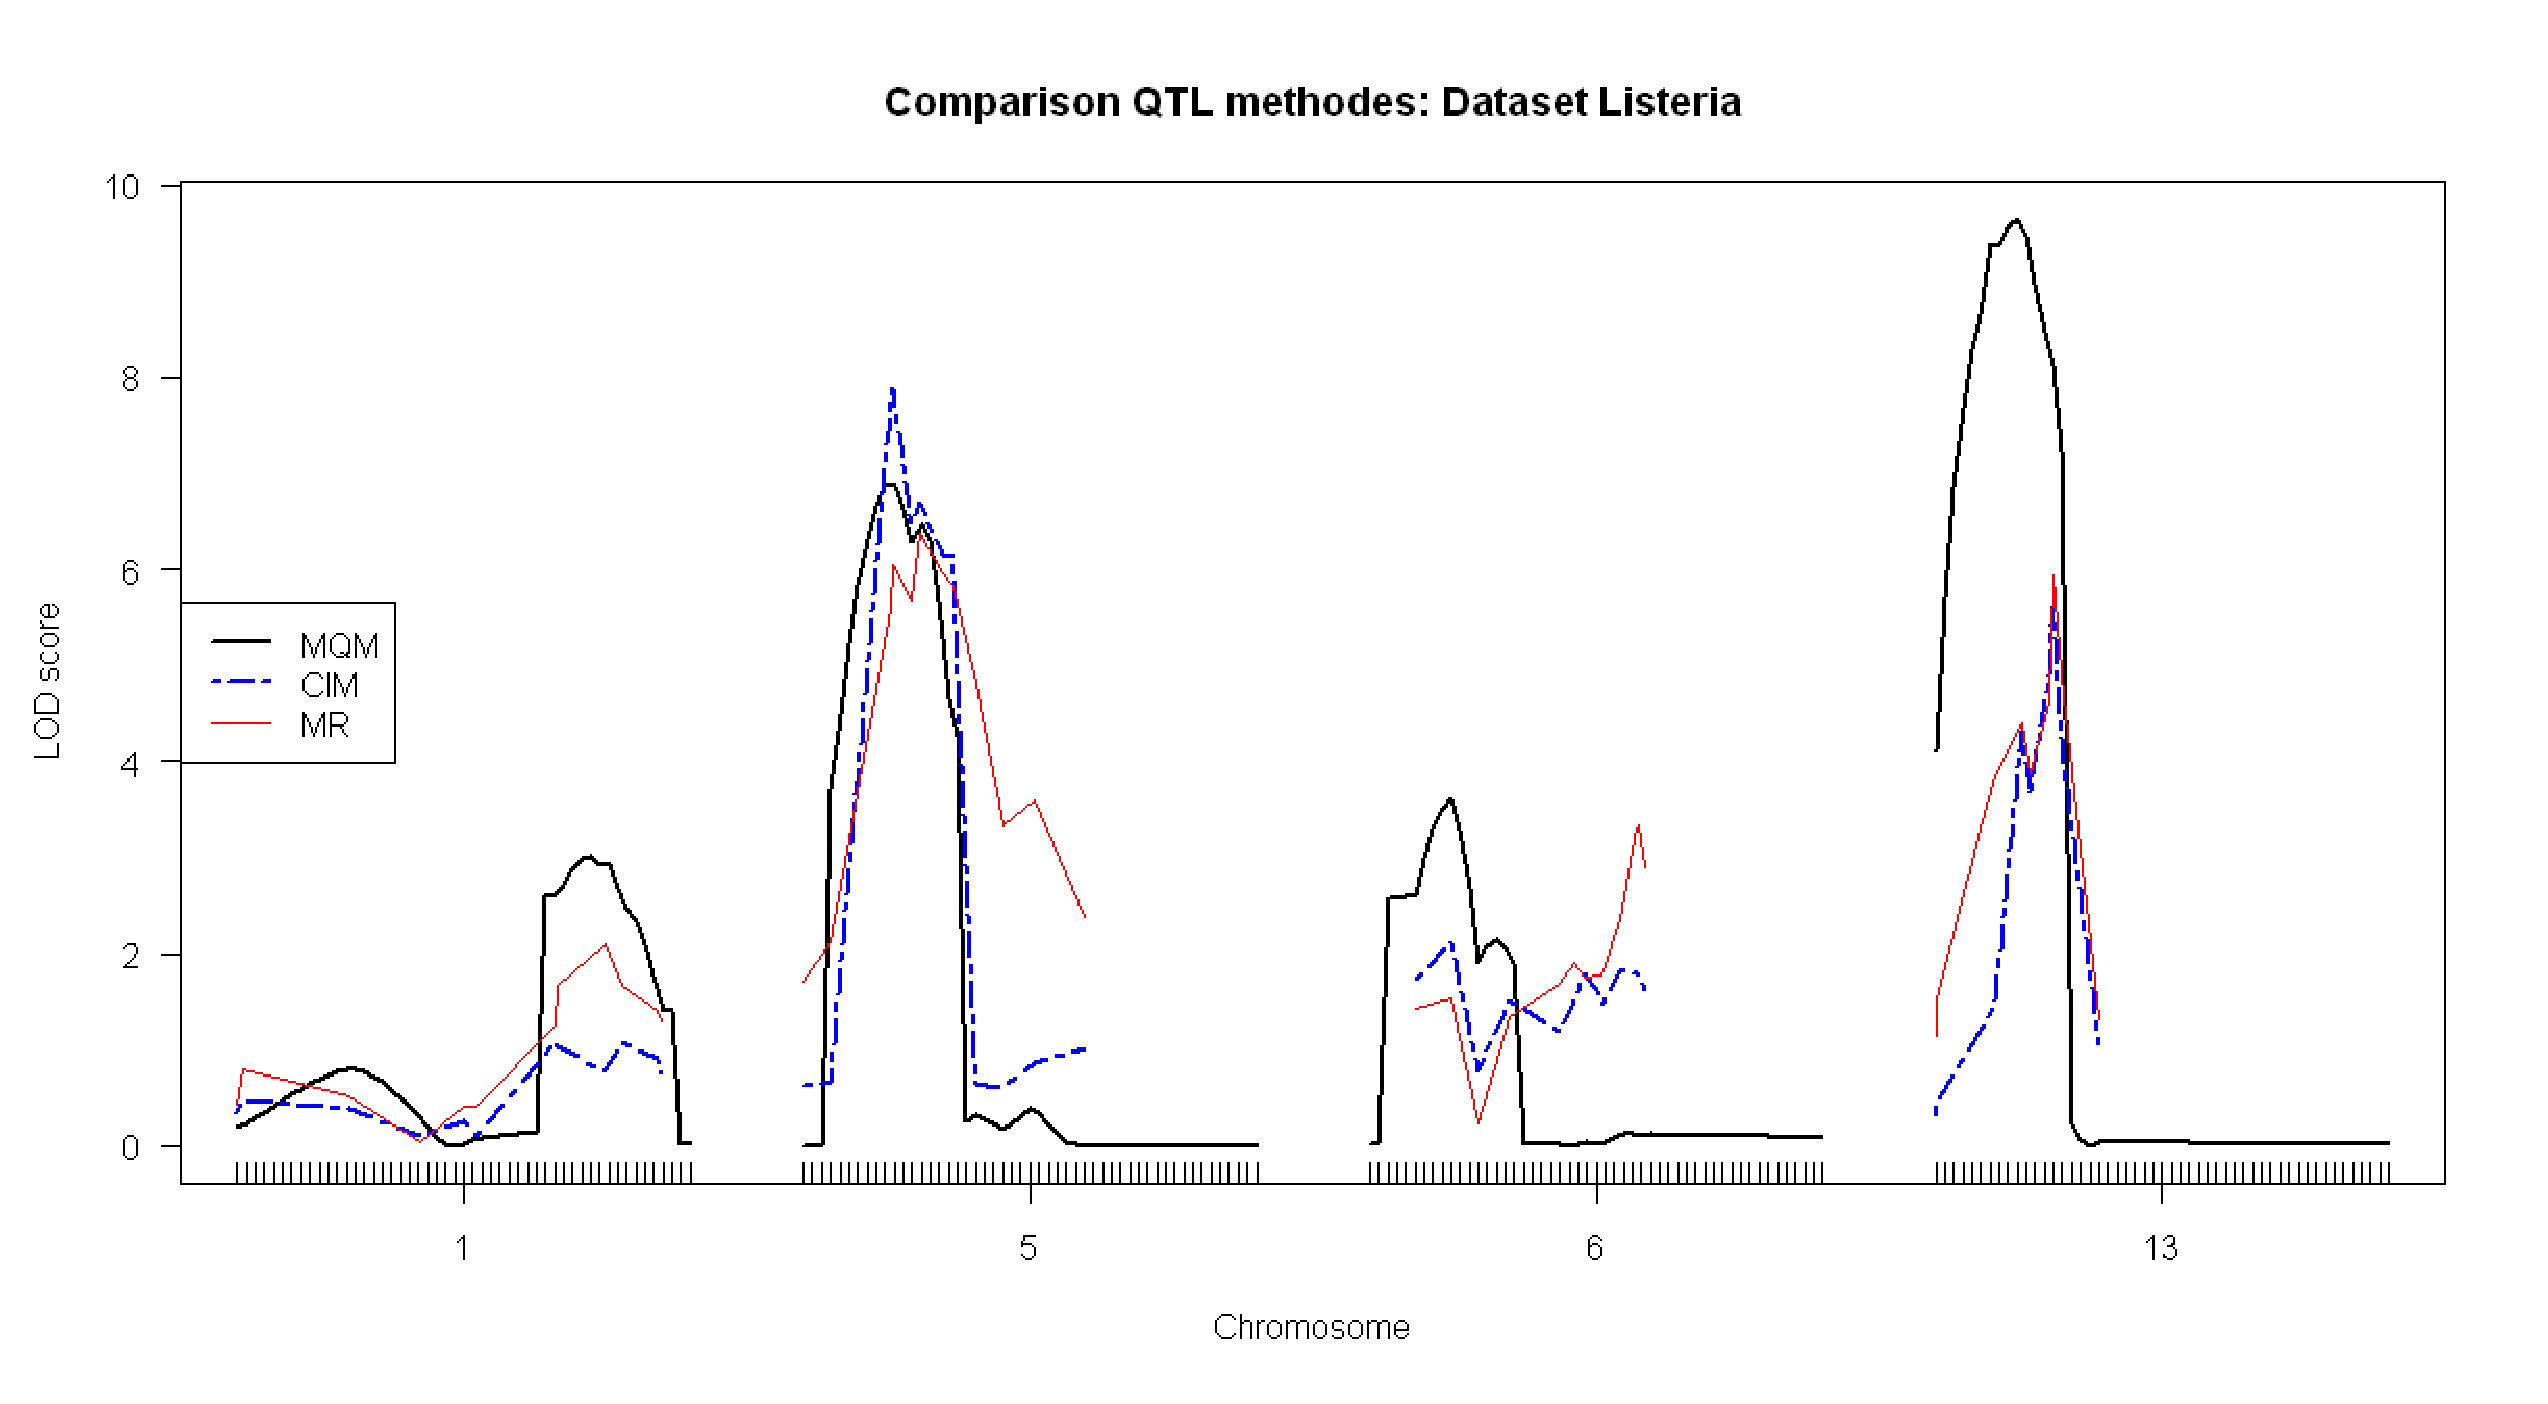
\includegraphics[height=8.0cm,width=12.0cm]{Images/DatasetListeria.eps}}
	  \label{fig:FigureListeria}
	  \caption{MQM in comparison with other QTLmapping methods (CIM, MR) using the dataset: \"listeria\". Using MQM we set cofactors every even marker, and do backward selection using a windowsize of 15 Cm. CIM also uses a window of 15Cm}
	\end{figure}
	
	\begin{figure}[ht]
	  \hfill
	  \fbox{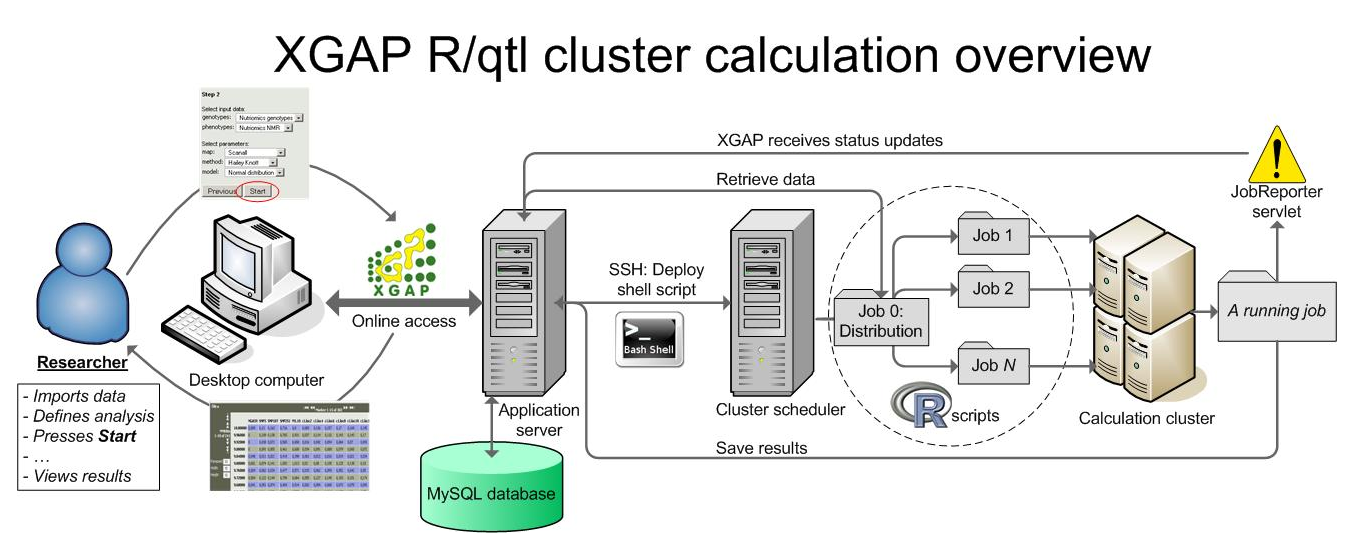
\includegraphics[height=6.0cm,width=12.0cm]{Images/Cluster_Layout.eps}}
	  \label{fig:FigureCluster}
	  \caption{Clusterlayout used at GBIC to do HPC analysis of QTLs using an opteroncluster controlled from the webinterface of a molgenis databaseserver}
	\end{figure}
	
	\begin{figure}[ht]
	  \hfill
	  \fbox{\includegraphics[height=6.0cm,width=12.0cm]{Images/taskviewer.eps}}
	  \label{fig:FigureTaskman}
	  \caption{Overview of the tasmanager plugin. Seen here are different tasks that have been submitted to the cluster. For an overview of the statuscolors see table \ref{tbl:tabelSTATUS}}
	\end{figure}